
\section*{Revisjonshistorie}
\begin{center}
 \begin{tabular}{|p{1.5cm} p{5.5cm}|} 
 \hline
 År & Forfatter \\ [0.5ex] 
 \hline\hline
 2016 & Konstanze Kölle  \\ 
 \hline
 2020 & Kolbjørn Austreng  \\ 
 \hline
 2021 & Kiet Tuan Hoang \\
 \hline
 2022 & Kiet Tuan Hoang \\
 \hline
\end{tabular}
\end{center}


\begin{alphasection}
\section{Praktisk rundt filene}

I denne laben får dere ikke utlevert noen \verb|.c| eller \verb|.h|-filer så dere trenger ikke å bry dere om det.



\section{Introduksjon - Praktisk rundt labben}
PLS (\textbf{P}rogrammerbar \textbf{L}ogisk \textbf{S}tyringsenhet) er et utbredt verktøy for å løse automatiseringsoppgaver i industrien. En PLS er en forholdsvis enkel innretning, som består av en prosessor, digitale- og/eller analoge innganger, og eventuelt også en eller flere kommunikasjonsgrensesnitt.

I praksis vil man koble en rekke sensorer (fotoceller, endebrytere, nivåfølere, etc) til PLSens innganger, og en rekke pådragsorganer (motorer, ventiler, lamper, releer, etc) til PLSens utganger. På selve PLSen implementerer man et sett med logiske funksjoner, slik at man kan sette utgangene basert på hva som inngangene registrerer. Disse logiske funksjonene kan være rent kombinatoriske funksjsoner, sekvensielle funksjoner, eller en blanding av de to.

I denne labben skal vi bruke en PLS fra SIemens kalt SIMATIC S7-300. Dette er en PLS som ble introdusert i 1994, sammen med lillebroren S7-200 og storebroren S7-400. Med disse systemene ble også den nye feltbusstandarden "PROFIBUS" og industrielt ethernett introdusert - som markerte starten på "nettverksalderen" for PLS. 


I bunn og grunn er PLSer så enkle at "ingenting" kan gå ordentlig galt. Om man trenger å implementere et automatisk styresystem for et industrielt anlegg, som skal stå i 20 år uten omstart, da er en PLS et godt egnet verktøy. Hadde man prøvd å styre det samme anlegget med en Windows-maskin, ville anlegget krevd en omstart i uka, hackere hadde vært inne allerede ved lanseringsdatoen, og om et par år må man kjøpe en ny lisens.

\subsection*{Vurdering}



PLS-labben er konseptuelt delt inn i to deler, hvor siste del er frivillig for de spesielt interessert. I første del skal dere programmere PLS med funksjonsblokkdiagrammer, som er et standarisert grafisk programmeringsspråk for PLSer. Oppgavene som handler om funksjonsblokkdiagrammer finner dere i seksjon \ref{sec:3-oppgave1}. Deretter skal dere få kjennskap til å programmere med sekvensielle funksjonsdiagrammer, som er nok et standarisert grafisk programmeringsspråk for PLSer slik som vanlige funksjonsblokkdiagrammer, men har i tillegg noen elementer for å kunne blande sekvensielle operasjoner med parallelle operasjoner. Oppgavene som handler om sekvensielle funksjonsblokkdiagrammer finner dere i seksjon \ref{sec:4-oppgave} og er som sagt frivillige. Det er viktig å merke seg at programmet for å kjøre PLSen er installert på Windows, og ikke på Ubuntu for datamaskinene i sanntidssalen.






\section{Introduksjon - Heisen på Sanntidslabben}\label{sec:1-intro}



I figur \ref{fig:siemens-pls} ser dere PLSen brukt på Sanntidssalen. Dette er en modulbasert PLS, som betyr at PLSens funksjonaliteter kan utvides ved behov, ved å legge til ekstra moduler. Det er faktisk bare "klossen" som har et 2-tall nede i venstre hjørne som er selve PLSen. Den første klossen er strømforsyning, og de tre andre er moduler som kan gjøre Input/Output. 

\begin{figure}[ht]
    \centering
    \includegraphics[scale=0.45]{figures/siemens.PNG}
    \caption{PLSen på Sanntidslabben.}
    \label{fig:siemens-pls}
\end{figure}

I tillegg, skal det på labplassen stå en del andre ting (se figur \ref{fig:Heis-modell}):


\begin{figure}[ht!]
    \centering
    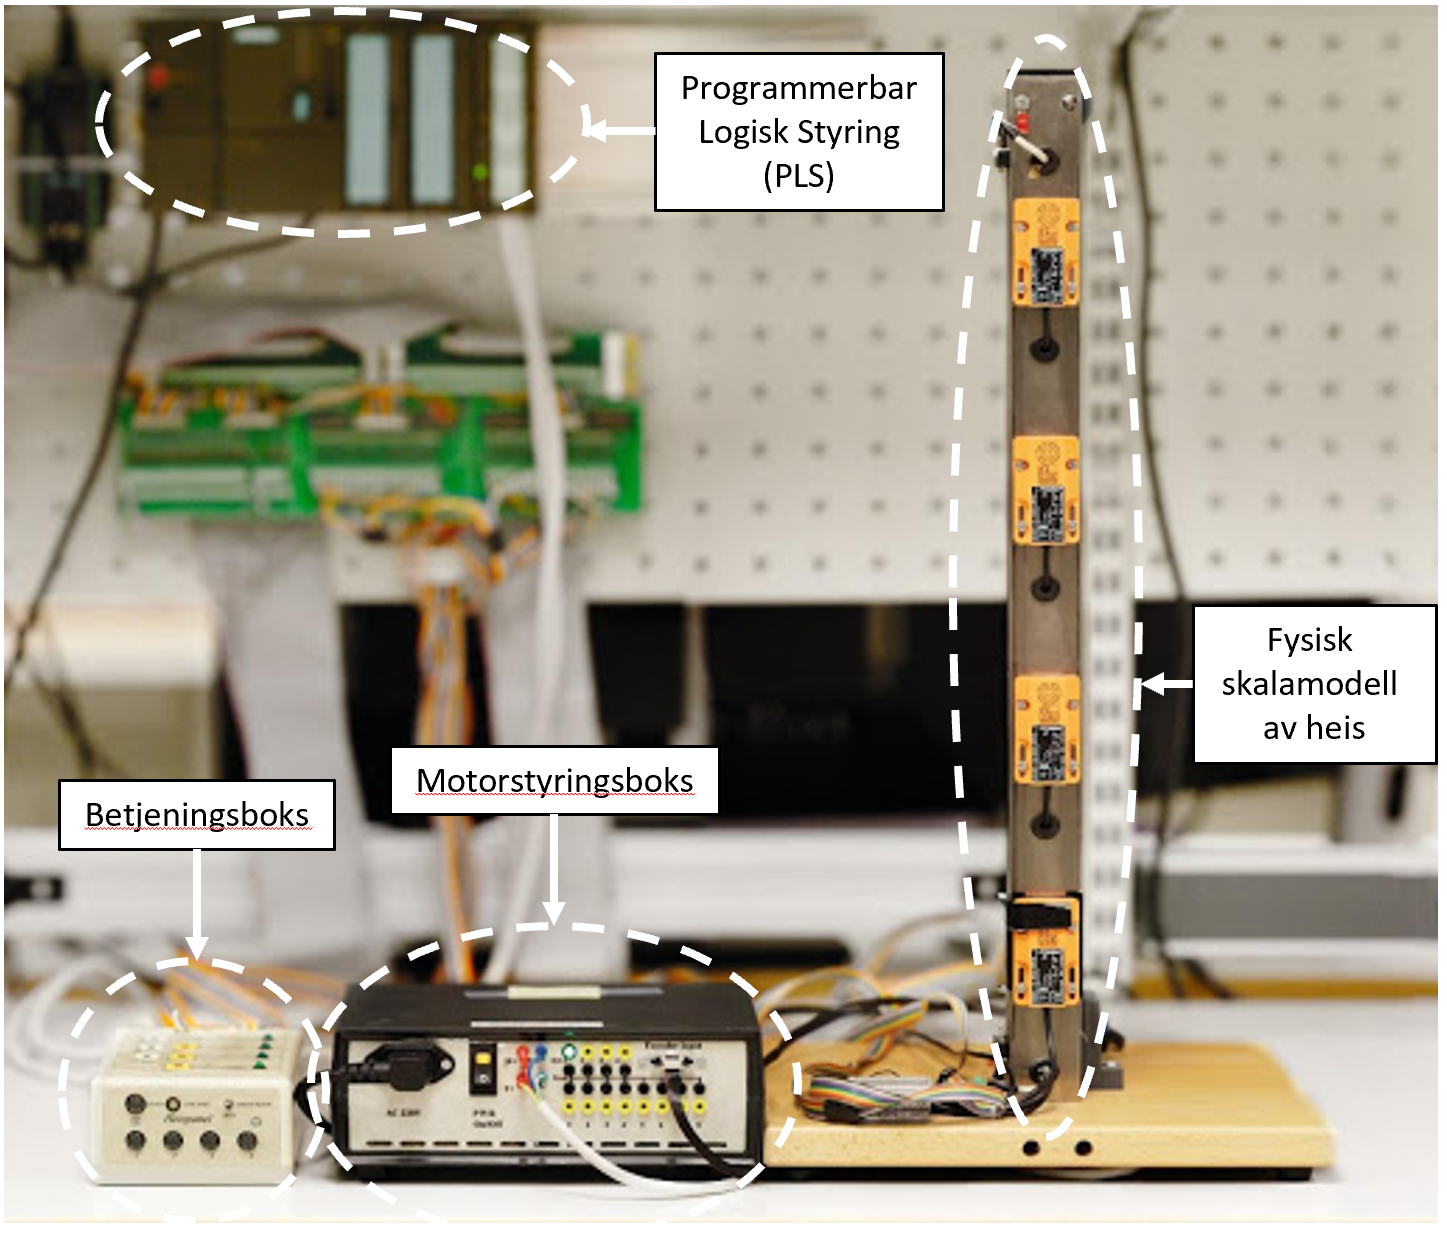
\includegraphics[scale=.85]{figures/heis.PNG}
    \caption{Heis-modellen på Sanntidslabben.}
    \label{fig:Heis-modell}
\end{figure}

\subsection{Heis-modell}

Dere skal ha en heis-modell, som består av en sjakt og en bevegelig heisstol. Det er denne vi skal få til å bevege seg i labopplegget. Over øverste etasje, og under nederste etasje er det montert endestoppbrytere, som vil kutte motorpådraget dersom heisen kjører utenfor sitt lovlige område. Dette er for å beskytte heisens motor mot skade. Om heisen skulle treffe en av endestoppene, må heisstolen manuelt skyves bort fra bryterne før en kan be motoren om et nytt pådrag. Dette er en beskyttelsemekanisme i hardware og skal ikke inngå i selve styresystemet som skal bli utviklet i denne labben.



\subsection{Motorstyringsboks}
Heisens pådrag kommer fra en motordriver - dette er den store svarte boksen som står ved siden av heismodellen.  Motoren er utstyrt med innebygd strømforsyning og kraftforsterker. Veien motoren skal gå settes ved et ekstra retningsbit i styringsboksens grensesnitt. Alt dette gjøres via funksjonskall i styringsprogrammet. Før dere gjør noe annet, skrur dere denne på, og passer på at den røde ledningen fra heisen er koblet til \verb|M+|, og den blå ledningen til \verb|M-|.


\subsection{Betjeningsboks}
Til slutt har dere en "betjeningsboks". Øverst på betjeningsboksen finnes en bryter som velger om datamaskinen eller PLSen skal styre heismodellen. Denne skal stå i "\verb|PLS|" gjennom hele labben.



Dersom man ser nærmere på betjeningsboksen, kan man se at den består av et etasjepanel, og et heispanel (se figur \ref{fig:paneler}):

Etasjepanelet finnes på oversiden av betjeningsboksen fra figur \ref{fig:Heis-modell}. Dette panelet blir brukt for å simulere bestillingsknappene for opp- og nedretning fra hver etasje.  Hver av knappene er utstyrt med lys som skal indikerer om en bestilling er mottatt eller ei. Etasjepanelet har også ett lys for hver etasje for å indikere hvilken etasje heisen befinner seg i. Det finnes ingen kopling mellom knappene og lyssignalet i elektronikken så lyset må settes av styringssystemet.

Heispanelet derimot, finner man på kortsiden av betjeningsboksen og representerer de knappene man forventer å finne inn i heisrommet til en vanlig heis. Her har man bestillingsknapper for hver etasje, samt en stoppknapp for nødstans. Alle knappene er utstyrt med lys som kan settes via styreprogrammet. I tillegg til knappene er panelet utstyrt med etasjeindikatorlys som kan settes via styreprogrammet og et lys, markert med "\verb|Dør Åpen|", som indikerer om heisdøren er åpen. Heispanelet har også en obstruksjonsbryter, som kan brukes for å simulere at en person blokkerer døren når den er åpen.






\begin{figure}[ht!]
    \centering
    



\resizebox{1\textwidth}{!}{\tikzset{every picture/.style={line width=0.75pt}} %set default line width to 0.75pt        


\tikzset{every picture/.style={line width=0.75pt}} %set default line width to 0.75pt        

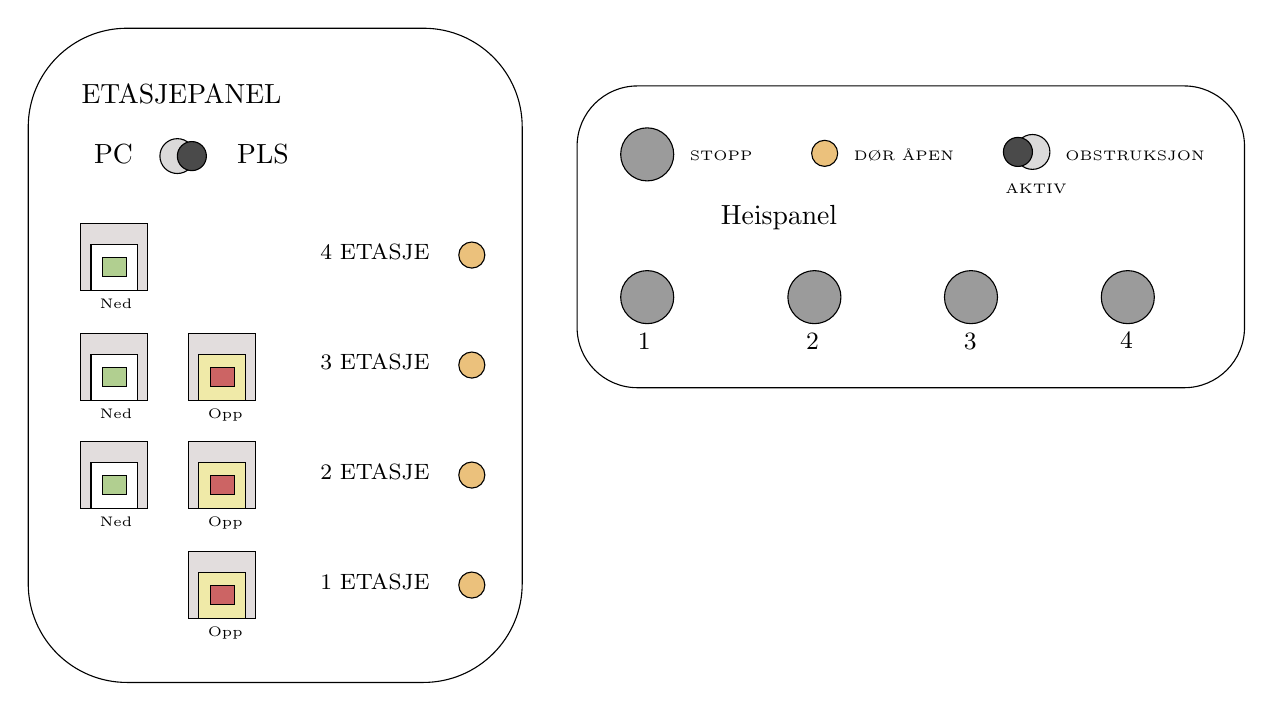
\begin{tikzpicture}[x=0.75pt,y=0.75pt,yscale=-1,xscale=1]
%uncomment if require: \path (0,386); %set diagram left start at 0, and has height of 386

%Rounded Rect [id:dp9950110832791259] 
\draw   (47.56,88.6) .. controls (47.56,62.31) and (68.87,41) .. (95.16,41) -- (237.96,41) .. controls (264.25,41) and (285.56,62.31) .. (285.56,88.6) -- (285.56,308.6) .. controls (285.56,334.89) and (264.25,356.2) .. (237.96,356.2) -- (95.16,356.2) .. controls (68.87,356.2) and (47.56,334.89) .. (47.56,308.6) -- cycle ;
%Shape: Circle [id:dp32702530949930675] 
\draw  [fill={rgb, 255:red, 219; green, 218; blue, 218 }  ,fill opacity=1 ] (111,102.6) .. controls (111,97.96) and (114.76,94.2) .. (119.4,94.2) .. controls (124.04,94.2) and (127.8,97.96) .. (127.8,102.6) .. controls (127.8,107.24) and (124.04,111) .. (119.4,111) .. controls (114.76,111) and (111,107.24) .. (111,102.6) -- cycle ;
%Shape: Circle [id:dp5550022005610891] 
\draw  [fill={rgb, 255:red, 74; green, 74; blue, 74 }  ,fill opacity=1 ] (119.4,102.6) .. controls (119.4,98.73) and (122.53,95.6) .. (126.4,95.6) .. controls (130.27,95.6) and (133.4,98.73) .. (133.4,102.6) .. controls (133.4,106.47) and (130.27,109.6) .. (126.4,109.6) .. controls (122.53,109.6) and (119.4,106.47) .. (119.4,102.6) -- cycle ;
%Rounded Rect [id:dp07742975412184872] 
\draw   (312,97.88) .. controls (312,81.82) and (325.02,68.8) .. (341.08,68.8) -- (604.48,68.8) .. controls (620.54,68.8) and (633.56,81.82) .. (633.56,97.88) -- (633.56,185.12) .. controls (633.56,201.18) and (620.54,214.2) .. (604.48,214.2) -- (341.08,214.2) .. controls (325.02,214.2) and (312,201.18) .. (312,185.12) -- cycle ;
%Shape: Circle [id:dp5584647222054995] 
\draw  [fill={rgb, 255:red, 155; green, 155; blue, 155 }  ,fill opacity=1 ] (333,101.78) .. controls (333,94.72) and (338.72,89) .. (345.78,89) .. controls (352.84,89) and (358.56,94.72) .. (358.56,101.78) .. controls (358.56,108.84) and (352.84,114.56) .. (345.78,114.56) .. controls (338.72,114.56) and (333,108.84) .. (333,101.78) -- cycle ;
%Shape: Circle [id:dp36378536676727435] 
\draw  [fill={rgb, 255:red, 235; green, 193; blue, 124 }  ,fill opacity=1 ] (425,101.28) .. controls (425,97.81) and (427.81,95) .. (431.28,95) .. controls (434.75,95) and (437.56,97.81) .. (437.56,101.28) .. controls (437.56,104.75) and (434.75,107.56) .. (431.28,107.56) .. controls (427.81,107.56) and (425,104.75) .. (425,101.28) -- cycle ;
%Shape: Circle [id:dp2626490795793748] 
\draw  [fill={rgb, 255:red, 219; green, 218; blue, 218 }  ,fill opacity=1 ] (523,100.6) .. controls (523,95.96) and (526.76,92.2) .. (531.4,92.2) .. controls (536.04,92.2) and (539.8,95.96) .. (539.8,100.6) .. controls (539.8,105.24) and (536.04,109) .. (531.4,109) .. controls (526.76,109) and (523,105.24) .. (523,100.6) -- cycle ;
%Shape: Circle [id:dp7325663462799819] 
\draw  [fill={rgb, 255:red, 74; green, 74; blue, 74 }  ,fill opacity=1 ] (517.4,100.6) .. controls (517.4,96.73) and (520.53,93.6) .. (524.4,93.6) .. controls (528.27,93.6) and (531.4,96.73) .. (531.4,100.6) .. controls (531.4,104.47) and (528.27,107.6) .. (524.4,107.6) .. controls (520.53,107.6) and (517.4,104.47) .. (517.4,100.6) -- cycle ;

%Shape: Circle [id:dp3804510595811603] 
\draw  [fill={rgb, 255:red, 155; green, 155; blue, 155 }  ,fill opacity=1 ] (333,170.56) .. controls (333,163.5) and (338.72,157.78) .. (345.78,157.78) .. controls (352.84,157.78) and (358.56,163.5) .. (358.56,170.56) .. controls (358.56,177.62) and (352.84,183.34) .. (345.78,183.34) .. controls (338.72,183.34) and (333,177.62) .. (333,170.56) -- cycle ;
%Shape: Circle [id:dp9317202699472626] 
\draw  [fill={rgb, 255:red, 155; green, 155; blue, 155 }  ,fill opacity=1 ] (413.56,170.56) .. controls (413.56,163.5) and (419.28,157.78) .. (426.34,157.78) .. controls (433.4,157.78) and (439.12,163.5) .. (439.12,170.56) .. controls (439.12,177.62) and (433.4,183.34) .. (426.34,183.34) .. controls (419.28,183.34) and (413.56,177.62) .. (413.56,170.56) -- cycle ;
%Shape: Circle [id:dp8967657062909633] 
\draw  [fill={rgb, 255:red, 155; green, 155; blue, 155 }  ,fill opacity=1 ] (489,170.56) .. controls (489,163.5) and (494.72,157.78) .. (501.78,157.78) .. controls (508.84,157.78) and (514.56,163.5) .. (514.56,170.56) .. controls (514.56,177.62) and (508.84,183.34) .. (501.78,183.34) .. controls (494.72,183.34) and (489,177.62) .. (489,170.56) -- cycle ;
%Shape: Circle [id:dp46875668862956843] 
\draw  [fill={rgb, 255:red, 155; green, 155; blue, 155 }  ,fill opacity=1 ] (564.56,170.56) .. controls (564.56,163.5) and (570.28,157.78) .. (577.34,157.78) .. controls (584.4,157.78) and (590.12,163.5) .. (590.12,170.56) .. controls (590.12,177.62) and (584.4,183.34) .. (577.34,183.34) .. controls (570.28,183.34) and (564.56,177.62) .. (564.56,170.56) -- cycle ;
%Shape: Circle [id:dp6506882141668844] 
\draw  [fill={rgb, 255:red, 235; green, 193; blue, 124 }  ,fill opacity=1 ] (255,150.28) .. controls (255,146.81) and (257.81,144) .. (261.28,144) .. controls (264.75,144) and (267.56,146.81) .. (267.56,150.28) .. controls (267.56,153.75) and (264.75,156.56) .. (261.28,156.56) .. controls (257.81,156.56) and (255,153.75) .. (255,150.28) -- cycle ;
%Shape: Circle [id:dp7349408120329506] 
\draw  [fill={rgb, 255:red, 235; green, 193; blue, 124 }  ,fill opacity=1 ] (255,203.28) .. controls (255,199.81) and (257.81,197) .. (261.28,197) .. controls (264.75,197) and (267.56,199.81) .. (267.56,203.28) .. controls (267.56,206.75) and (264.75,209.56) .. (261.28,209.56) .. controls (257.81,209.56) and (255,206.75) .. (255,203.28) -- cycle ;
%Shape: Circle [id:dp08591264771647289] 
\draw  [fill={rgb, 255:red, 235; green, 193; blue, 124 }  ,fill opacity=1 ] (255,256.28) .. controls (255,252.81) and (257.81,250) .. (261.28,250) .. controls (264.75,250) and (267.56,252.81) .. (267.56,256.28) .. controls (267.56,259.75) and (264.75,262.56) .. (261.28,262.56) .. controls (257.81,262.56) and (255,259.75) .. (255,256.28) -- cycle ;
%Shape: Circle [id:dp13492097445361106] 
\draw  [fill={rgb, 255:red, 235; green, 193; blue, 124 }  ,fill opacity=1 ] (255,309.28) .. controls (255,305.81) and (257.81,303) .. (261.28,303) .. controls (264.75,303) and (267.56,305.81) .. (267.56,309.28) .. controls (267.56,312.75) and (264.75,315.56) .. (261.28,315.56) .. controls (257.81,315.56) and (255,312.75) .. (255,309.28) -- cycle ;
%Shape: Square [id:dp9156786654213831] 
\draw  [fill={rgb, 255:red, 226; green, 221; blue, 221 }  ,fill opacity=1 ] (72.8,135) -- (105,135) -- (105,167.2) -- (72.8,167.2) -- cycle ;
%Shape: Rectangle [id:dp9366523430197387] 
\draw  [color={rgb, 255:red, 0; green, 0; blue, 0 }  ,draw opacity=1 ][fill={rgb, 255:red, 255; green, 255; blue, 255 }  ,fill opacity=1 ] (77.8,145.2) -- (100.24,145.2) -- (100.24,167.2) -- (77.8,167.2) -- cycle ;
%Shape: Rectangle [id:dp17647947769063999] 
\draw  [fill={rgb, 255:red, 177; green, 207; blue, 144 }  ,fill opacity=1 ] (83.24,151.6) -- (94.8,151.6) -- (94.8,160.8) -- (83.24,160.8) -- cycle ;
%Shape: Square [id:dp3110641273660344] 
\draw  [fill={rgb, 255:red, 226; green, 221; blue, 221 }  ,fill opacity=1 ] (124.8,188) -- (157,188) -- (157,220.2) -- (124.8,220.2) -- cycle ;
%Shape: Rectangle [id:dp3411082188269683] 
\draw  [fill={rgb, 255:red, 240; green, 234; blue, 168 }  ,fill opacity=1 ] (129.8,198.2) -- (152.24,198.2) -- (152.24,220.2) -- (129.8,220.2) -- cycle ;
%Shape: Rectangle [id:dp024921669891114773] 
\draw  [fill={rgb, 255:red, 204; green, 100; blue, 100 }  ,fill opacity=1 ] (135.24,204.6) -- (146.8,204.6) -- (146.8,213.8) -- (135.24,213.8) -- cycle ;
%Shape: Square [id:dp802085856449118] 
\draw  [fill={rgb, 255:red, 226; green, 221; blue, 221 }  ,fill opacity=1 ] (124.8,240) -- (157,240) -- (157,272.2) -- (124.8,272.2) -- cycle ;
%Shape: Rectangle [id:dp5915145699519246] 
\draw  [fill={rgb, 255:red, 240; green, 234; blue, 168 }  ,fill opacity=1 ] (129.8,250.2) -- (152.24,250.2) -- (152.24,272.2) -- (129.8,272.2) -- cycle ;
%Shape: Rectangle [id:dp03960973210916041] 
\draw  [fill={rgb, 255:red, 204; green, 100; blue, 100 }  ,fill opacity=1 ] (135.24,256.6) -- (146.8,256.6) -- (146.8,265.8) -- (135.24,265.8) -- cycle ;
%Shape: Square [id:dp831298532737776] 
\draw  [fill={rgb, 255:red, 226; green, 221; blue, 221 }  ,fill opacity=1 ] (124.8,293) -- (157,293) -- (157,325.2) -- (124.8,325.2) -- cycle ;
%Shape: Rectangle [id:dp15467787894146512] 
\draw  [fill={rgb, 255:red, 240; green, 234; blue, 168 }  ,fill opacity=1 ] (129.8,303.2) -- (152.24,303.2) -- (152.24,325.2) -- (129.8,325.2) -- cycle ;
%Shape: Rectangle [id:dp34679432751904793] 
\draw  [fill={rgb, 255:red, 204; green, 100; blue, 100 }  ,fill opacity=1 ] (135.24,309.6) -- (146.8,309.6) -- (146.8,318.8) -- (135.24,318.8) -- cycle ;
%Shape: Square [id:dp4723272264815428] 
\draw  [fill={rgb, 255:red, 226; green, 221; blue, 221 }  ,fill opacity=1 ] (72.8,240) -- (105,240) -- (105,272.2) -- (72.8,272.2) -- cycle ;
%Shape: Rectangle [id:dp07462637657852489] 
\draw  [color={rgb, 255:red, 0; green, 0; blue, 0 }  ,draw opacity=1 ][fill={rgb, 255:red, 255; green, 255; blue, 255 }  ,fill opacity=1 ] (77.8,250.2) -- (100.24,250.2) -- (100.24,272.2) -- (77.8,272.2) -- cycle ;
%Shape: Rectangle [id:dp5263621720064795] 
\draw  [fill={rgb, 255:red, 177; green, 207; blue, 144 }  ,fill opacity=1 ] (83.24,256.6) -- (94.8,256.6) -- (94.8,265.8) -- (83.24,265.8) -- cycle ;
%Shape: Square [id:dp4171956285217089] 
\draw  [fill={rgb, 255:red, 226; green, 221; blue, 221 }  ,fill opacity=1 ] (72.8,188) -- (105,188) -- (105,220.2) -- (72.8,220.2) -- cycle ;
%Shape: Rectangle [id:dp8897782495872741] 
\draw  [color={rgb, 255:red, 0; green, 0; blue, 0 }  ,draw opacity=1 ][fill={rgb, 255:red, 255; green, 255; blue, 255 }  ,fill opacity=1 ] (77.8,198.2) -- (100.24,198.2) -- (100.24,220.2) -- (77.8,220.2) -- cycle ;
%Shape: Rectangle [id:dp3645531927882917] 
\draw  [fill={rgb, 255:red, 177; green, 207; blue, 144 }  ,fill opacity=1 ] (83.24,204.6) -- (94.8,204.6) -- (94.8,213.8) -- (83.24,213.8) -- cycle ;

% Text Node
\draw (72,67) node [anchor=north west][inner sep=0.75pt]   [align=left] {ETASJEPANEL};
% Text Node
\draw (78,96) node [anchor=north west][inner sep=0.75pt]   [align=left] {PC};
% Text Node
\draw (147,96) node [anchor=north west][inner sep=0.75pt]   [align=left] {PLS};
% Text Node
\draw (380.05,124.81) node [anchor=north west][inner sep=0.75pt]   [align=left] {Heispanel};
% Text Node
\draw (444.05,97.81) node [anchor=north west][inner sep=0.75pt]  [font=\tiny] [align=left] {DØR ÅPEN};
% Text Node
\draw (546.05,98.81) node [anchor=north west][inner sep=0.75pt]  [font=\tiny] [align=left] {OBSTRUKSJON};
% Text Node
\draw (365.05,98.81) node [anchor=north west][inner sep=0.75pt]  [font=\tiny] [align=left] {STOPP};
% Text Node
\draw (517.05,114.81) node [anchor=north west][inner sep=0.75pt]  [font=\tiny] [align=left] {AKTIV};
% Text Node
\draw (340.05,186.81) node [anchor=north west][inner sep=0.75pt]  [font=\small] [align=left] {1};
% Text Node
\draw (421.05,186.81) node [anchor=north west][inner sep=0.75pt]  [font=\small] [align=left] {2};
% Text Node
\draw (497.05,186.81) node [anchor=north west][inner sep=0.75pt]  [font=\small] [align=left] {3};
% Text Node
\draw (572.34,186.34) node [anchor=north west][inner sep=0.75pt]  [font=\small] [align=left] {4};
% Text Node
\draw (187,144) node [anchor=north west][inner sep=0.75pt]  [font=\footnotesize] [align=left] {4 ETASJE};
% Text Node
\draw (187,197) node [anchor=north west][inner sep=0.75pt]  [font=\footnotesize] [align=left] {3 ETASJE};
% Text Node
\draw (187,250) node [anchor=north west][inner sep=0.75pt]  [font=\footnotesize] [align=left] {2 ETASJE};
% Text Node
\draw (187,303) node [anchor=north west][inner sep=0.75pt]  [font=\footnotesize] [align=left] {1 ETASJE};
% Text Node
\draw (80.8,170.2) node [anchor=north west][inner sep=0.75pt]  [font=\tiny] [align=left] {Ned};
% Text Node
\draw (80.8,223.2) node [anchor=north west][inner sep=0.75pt]  [font=\tiny] [align=left] {Ned};
% Text Node
\draw (80.8,275.2) node [anchor=north west][inner sep=0.75pt]  [font=\tiny] [align=left] {Ned};
% Text Node
\draw (132.8,223.2) node [anchor=north west][inner sep=0.75pt]  [font=\tiny] [align=left] {Opp};
% Text Node
\draw (132.8,275.2) node [anchor=north west][inner sep=0.75pt]  [font=\tiny] [align=left] {Opp};
% Text Node
\draw (132.8,328.2) node [anchor=north west][inner sep=0.75pt]  [font=\tiny] [align=left] {Opp};


\end{tikzpicture}}
    \caption{Etasje- og Heispanel i Sanntidslabben}
    \label{fig:paneler}
\end{figure}



\section{Introduksjon - Kort om programmering av PLS}

Måten man programmerer PLSer på er standarisert og følger en industristandard kalt \verb|IEC 61131-3|. Denne standarden definerer flere forskjellige måter man kan programmere/fortelle en PLS hva den skal gjøre. Fire av de vanligste av disse er:

\begin{itemize}
    \item \verb|Stigediagram (LD)|, eller "Ladder diagram": er et grafisk programmeringsspråk, hvor man lager linjer som representerer programflyt, hvor linjene kan ha brytere som representerer kontrollstrukturerer.
    
    \item \verb|Funksjonsblokkdiagram (FBD)|: er også et grafisk programmeringsspråk, men her trekker man koblinger mellom utgangen på blokker inn i inngangene til andre blokker. 
    \item \verb|Strukturerert tekst (ST)|: er et programmeringsspråk som faktisk bruker tekjst - som navnet tilsier. Det ligner på et språk som heter "PASCAL".
    
    \item \verb|Sekvensielle funksjonsdiagram (SFC)| eller "Sequential function chart": er nok et grafisk programmeringsspråk, men har i tillegg noen elementer for å kunne blande sekvensielle operasjoner med parallelle operasjoner.
\end{itemize}

Programpakken som skal brukes heter SIMATIC STEP 7 (S7). Manualen for denne finner dere i \verb|STEP 7 - Working with STEP 7|. Denne finner dere i den utleverte mappen. I tillegg så finner dere en kopi på sanntidssalen. Grunnbjelken for denne programpakken er SIMATIC Manager og med denne kan man: 

\begin{itemize}
    \item Sette opp og organisere prosjekter
    \item Konfigurere hardware
    \item Programmere blokker
    \item Laste ned program til PLSen
    \item Debugge programmet online
    \item Starte opp tilhørende S7-verktøy
\end{itemize}

S7 støtter alle programmeringsspråkene i den internasjonale standarden. I denne laben skal vi imidlertid bare fokusere på funksjonsdiagrammer og sekvensielle funksjonsdiagrammer.

\subsection{Innføring i bruken av S7}

Det første man gjør når man skal programmere en PLS med STEP 7 er å opprette et prosjekt. Prosjektet er organisert som en mappestruktur. Mappene inneholder blant annet hardwarekonfigurasjonen, programblokker, og andre spesielle blokker som brukes under utvikling.

\subsubsection{Hardware}

PLS er et modulbasert system. I hardwarekonfigurasjonen angir vi hvilke fysiske enheter
PLSen er bygd opp av. Typisk kan dette være strømforsyning, prosessor, analoge og digitale
inn-/ut-enheter, kommunikasjonsenheter og feltinstrumenter med mere. Vi kan velge om vi vil
gjøre hardwarekonfigurasjonen før eller etter selve programmeringen.

\subsubsection{Software}

For å gjøre programstrukturen oversiktlig, er programmet organisert i blokker. I tillegg til egendefinerte blokker, finnes det også systemblokker som ligger ferdige i biblioteket. Relevante hovedtyper av blokker for denne laben finner man under:

\begin{itemize}
    \item \verb|Organisasjonsblokker| (\verb|OB|) representerer grensesnittet mellom operativsystemet og
brukerprogrammet. Disse blokkene kalles av operativsystemet. Vi skal i denne laboppgaven
kun bruke \verb|OB1|, en organisasjonsblokk som kjøres syklisk. I \verb|OB1| leses alle innganger før
beregningene utføres og alle utganger settes ut til de fysiske enhetene. Dette gjentar seg et
visst antall ganger pr. tidsenhet. Andre organisasjonsblokker kjøres kun ved avbrudd
(interrupt), ved oppstart eller ved deteksjon av feil.
\item \verb|Funksjoner| (\verb|FC|) er egendefinerte programdeler som brukes for å få en oversiktlig struktur
eller for programdeler som gjentar seg ofte. Funksjoner må kalles fra \verb|OB|, \verb|FC| eller \verb|FB| for at
de skal bli utført.
\item \verb|Funksjonsblokker| (\verb|FB|) likner funksjoner, men har i tillegg en datablokk som kan lagre data
mellom kallene.
\item \verb|Datablokker| (\verb|DB|) brukes til å lagre data.
\end{itemize}




Det er viktig at man ikke blander de 4 standardspråkene (\verb|LD, FBD, ST| eller \verb|SFC|) for en og samme blokk. Ellers står man fritt til å velge hvilke man vil bruke når man skriver blokkene. Blokkene er inndelte i nummererte nettverk, som er hvor programmet ligget. Dersom man bruker et av de grafisk baserte språkene, kan man enkelt velge programmeringselementene fra en meny, og deretter kople dem sammen. Se appendiks \ref{app:FB-elementer} for en oversikt over programmeringselementene vi får bruk for i denne laboppgaven. I tillegg til disse finnes det også en mengde andre programmeringselementer.





\section{Introduksjon - Interface med PLS}\label{subsec:intefrace}

Innganger og utganger blir i en PLS tildelt adresser, avhengig av hvor de er koblet i PLSens moduler. Adresser ser slik ut:

\begin{center}
 {\begin{tabular}{|c| c|} 
 \toprule
 \verb|Ix.y| & Adressen til input bit nummer \verb|y|, i
byte nummer \verb|x|.\\ 
 \toprule
 \verb|IBx| & Adressen til input byte nummer \verb|x|.  \\
 \toprule
 \verb|IWx| & Adressen til input word nummer \verb|x|.
(Et word er 32 bit)  \\

 \toprule
\end{tabular}}
\end{center}


Utgangene blir adressert på samme måte, men med prefiks “\verb|Q|” isteden for “\verb|I|”. Internt minne
adresseres også på samme måte, men med prefiks “\verb|M|”. Noen av I/O-adressene refereres som
“peripheral” og får en “\verb|P|” som første tegn (for eksempel \verb|PQW272| som i denne laboppgaven er
pådragssignalet til motoren). Se appendiks \ref{app:adresse} for nærmere detaljer om adresser.


For leseligheten av programmet vil det være en fordel om man bruker symbolske navn på
funksjoner og variabler. “Motor” er for eksempel lettere å forstå enn \verb|PQW272|. Alle symbolske navn
legges i “Symboltabellen”.

\subsection{Digital IO}

De digitale signalene til og fra heisen er samlet i to 25-pins D-kontakter på boksen til
betjeningstavlene. Fra D-kontaktene er det laget en fast kabel til de digitale inn- og utgangene
på PLSen. Dette medfører at hvert signal får en bestemt adresse i PLSen. Relevante addresser finner dere under:


\begin{center}
 {\begin{tabular}{|c| c|} 
 \hline
 \textbf{Minneadresse} & \textbf{Beskrivelse} \\ 
 \toprule
 \verb|I 8.0| & Obstruksjon \\ 
 \hline
 \verb|I 8.1| & Stopp-knapp \\ 
 \hline
 \verb|I 8.2| & H1 - Bestillingsknapp nr. 1 inne i heisen \\ 
 \hline
 \verb|I 8.3| & H1 - Bestillingsknapp nr. 2 inne i heisen \\ 
 \hline
 \verb|I 8.4| & H1 - Bestillingsknapp nr. 3 inne i heisen \\ 
 \hline
 \verb|I 8.5| & H1 - Bestillingsknapp nr. 4 inne i heisen \\ 
 \hline
 \verb|I 8.6| & Opp-knapp i etasje 1 \\ 
 \hline
 \verb|I 8.7| & Opp-knapp i etasje 2 \\ 
 \toprule
 
 \verb|I 9.0| & Ned-knapp i etasje 2 \\ 
 \hline
 \verb|I 9.1| & Opp-knapp i etasje 3 \\ 
 \hline
 \verb|I 9.2| & Ned-knapp i etasje 3\\ 
 \hline
 \verb|I 9.3| & Ned-knapp i etasje 4 \\ 
 \hline
 \verb|I 9.4| & Føler 1. etasje \\ 
 \hline
 \verb|I 9.5| & Føler 2. etasje \\ 
 \hline
 \verb|I 9.6| & Føler 3. etasje \\ 
 \hline
 \verb|I 9.7| & Føler 4. etasje \\ 
 \toprule
 
 \verb|Q 8.0| & DIR - Retning på motor (Opp=0, Ned=1) \\ 
 \hline
 \verb|Q 8.1| & Lys i stopp-knapp \\ 
 \hline
 \verb|Q 8.2| & Lys i bestillingsknapp nr. 1 \\ 
 \hline
 \verb|Q 8.3| & Lys i bestillingsknapp nr. 2 \\ 
 \hline
 \verb|Q 8.4| & Lys i bestillingsknapp nr. 3\\ 
 \hline
 \verb|Q 8.5| & Lys i bestillingsknapp nr. 4\\ 
 \hline
 \verb|Q 8.6| & Lys i opp-knapp i etasje 1 \\ 
 \hline
 \verb|Q 8.7| & Lys i opp-knapp i etasje 2 \\ 
 \toprule
 
 \verb|Q 9.0| & Lys i ned-knapp i etasje 2 \\ 
 \hline
 \verb|Q 9.1| &Lys i opp-knapp i etasje 3 \\ 
 \hline
 \verb|Q 9.2| & Lys i ned-knapp i etasje 3\\ 
 \hline
 \verb|Q 9.3| & Lys i ned-knapp i etasje 4\\ 
 \hline
 \verb|Q 9.4| & Lys i indikator for åpen dør \\ 
 \hline
 \verb|Q 9.5| &Ubrukt \\ 
 \hline
 \verb|Q 9.6| &Etasjeindikator bit 1 \\ 
 \hline
 \verb|Q 9.7| &Etasjeindikator bit 2 \\ 
 \toprule
\end{tabular}}
\end{center}

Fra tabellen over, kan man se at man bare har to bit for å sette etasjeindikatorlysene. Dette er for spare utganger på PLSen. I vårt tilfelle, er lyset kodet slik:

\begin{center}
 {\begin{tabular}{|c| c| c|} 
 \hline
 \textbf{Bit 2} & \textbf{Bit 1} & \textbf{Etasjeindikator lys} \\ 
 \toprule
 0 & 0 & Etasje 1 \\ 
 \hline
 0 & 1 & Etasje 2 \\
 \hline
 1 & 0 & Etasje 3 \\
 \hline
 1 & 1 & Etasje 4 \\
 \toprule
\end{tabular}}
\end{center}


\subsection{Analog IO}

I tillegg til de digitale IO, har vi et analogt output i form av pådragssignalet til motoren. Dette signalet har følgende addresse på PLSen:

\begin{center}
 {\begin{tabular}{|c| c|} 
 \hline
 \textbf{Minneadresse} & \textbf{Beskrivelse} \\ 
 \toprule
 \verb|PQW 272| & Motorpådrag \\ 
 \toprule
\end{tabular}}
\end{center}

Dette er en "periferi-output", og har da prefikset \verb|P|. Vi ønsker at dette pådragssignal skal ligge i området 0 - 5 \si{\V}. For å sette pådragssignalet til rett spenningsverdi bruker man for eksempel disse verdiene:

\begin{center}
 {\begin{tabular}{|c| c|} 
 \hline
 \textbf{Heksadesimal verdi} & \textbf{Spenningsverdi} \\ 
 \toprule
 \verb|W#16#0000| & 0.0 \si{\V} \\ 
 \hline
 \verb|W#16#3DFF| & 2.5 \si{\V}  \\
 \hline
 \verb|W#16#7EFF| & 5.0 \si{\V}  \\

 \toprule
\end{tabular}}
\end{center}



En enkel måte å sette ut det analoge signalet er å bruke \verb|MOVE|-blokken (se appendiks \ref{app:FB-elementer}).
\subsection{Simulert IO}

I tillegg til de fysiske digitale og analoge IO-linjene har vi også noen “simulerte” digitale IO-linjer. Disse ligger i modul nr. 4 i PLSen og har adressene \verb|I0.0-I0.7| og \verb|Q0.0-0.7|. Signalene
herfra er bare koplet til brytere/lysindikatorer på selve PLSen og kan for eksempel brukes til testing.




\end{alphasection}

\setcounter{section}{0}